%& -job-name=lesson1
\documentclass[10pt]{beamer}
%\documentclass[handout,10pt]{beamer}
%\mode<presentation>
%{
%  \usetheme{Berkeley}
%  \usecolortheme{seahorse}
%  \usefonttheme{default}  
%  \setbeamertemplate{navigation symbols}{}
%  \setbeamertemplate{caption}[numbered]
%} 

\usetheme{metropolis}

\usepackage[english]{babel}
\usepackage[utf8x]{inputenc}
\usepackage{caption}
\usepackage{multirow}
\usepackage{mathrsfs}
\usepackage{graphicx}
\usepackage{amsmath}
\usepackage{graphicx}
\usepackage[compatibility=false]{caption}
\usepackage{subcaption}
\usepackage[normalem]{ulem}
\DeclareMathOperator{\tr}{tr}
\usepackage{textpos}
\usepackage{animate}

\usepackage{tcolorbox}
\tcbset{colback=blue!5!white,colframe=blue!50!black}

\title[Computational Thinking]{Lesson 1: Computational Thinking Basics}
%\titlegraphic{\includegraphics[height=1.57cm]{logo.jpg}}
\author[Scott Morgan]{\textbf{Scott Morgan}}
\institute{\textit{Bridgend College}
	\\
	\textit{BTEC Computing: Computational Thinking (Unit 18)} \\ \\ \\
	\textit{Web: scott3142.com} \\ 
	\textit{E-mail: MorganSN@cardiff.ac.uk}}
\date

\begin{document}

\begin{frame}
	\maketitle
	\begin{textblock*}{2cm}(7.5cm,-3cm)
		
\includegraphics[height=1.57cm]{bcoll_logo.png}
	\end{textblock*}
\end{frame}

\begin{frame}{Computers Are Stupid!}

\begin{columns}	
	\begin{column}{0.5\textwidth}
		\begin{figure}[h]
			\centering
			
\includegraphics[scale=0.25]{stupid.jpg}
			\caption*{}
		\end{figure}
	\end{column}
	\begin{column}{0.5\textwidth}
		\begin{itemize}[<+->]
			\item Computers need to be \textit{programmed}.
			\item They cannot (yet) think for themselves.
			\item They speak a special language - \textit{binary}.
			\item They are highly \textit{logical}.
		\end{itemize}
	\end{column}
\end{columns}

\end{frame}

\begin{frame}{Recipes and Algorithms}

\begin{columns}	
	\begin{column}{0.5\textwidth}
		\begin{itemize}[<+->]
			\item Programs are like \textit{recipes}.
			\item Each instruction must lead to the next one.
			\item Nothing can be \textit{assumed}!
		\end{itemize}
	\end{column}
	\begin{column}{0.5\textwidth}
		\only<1-3>{
			\begin{figure}[h]
				\centering
				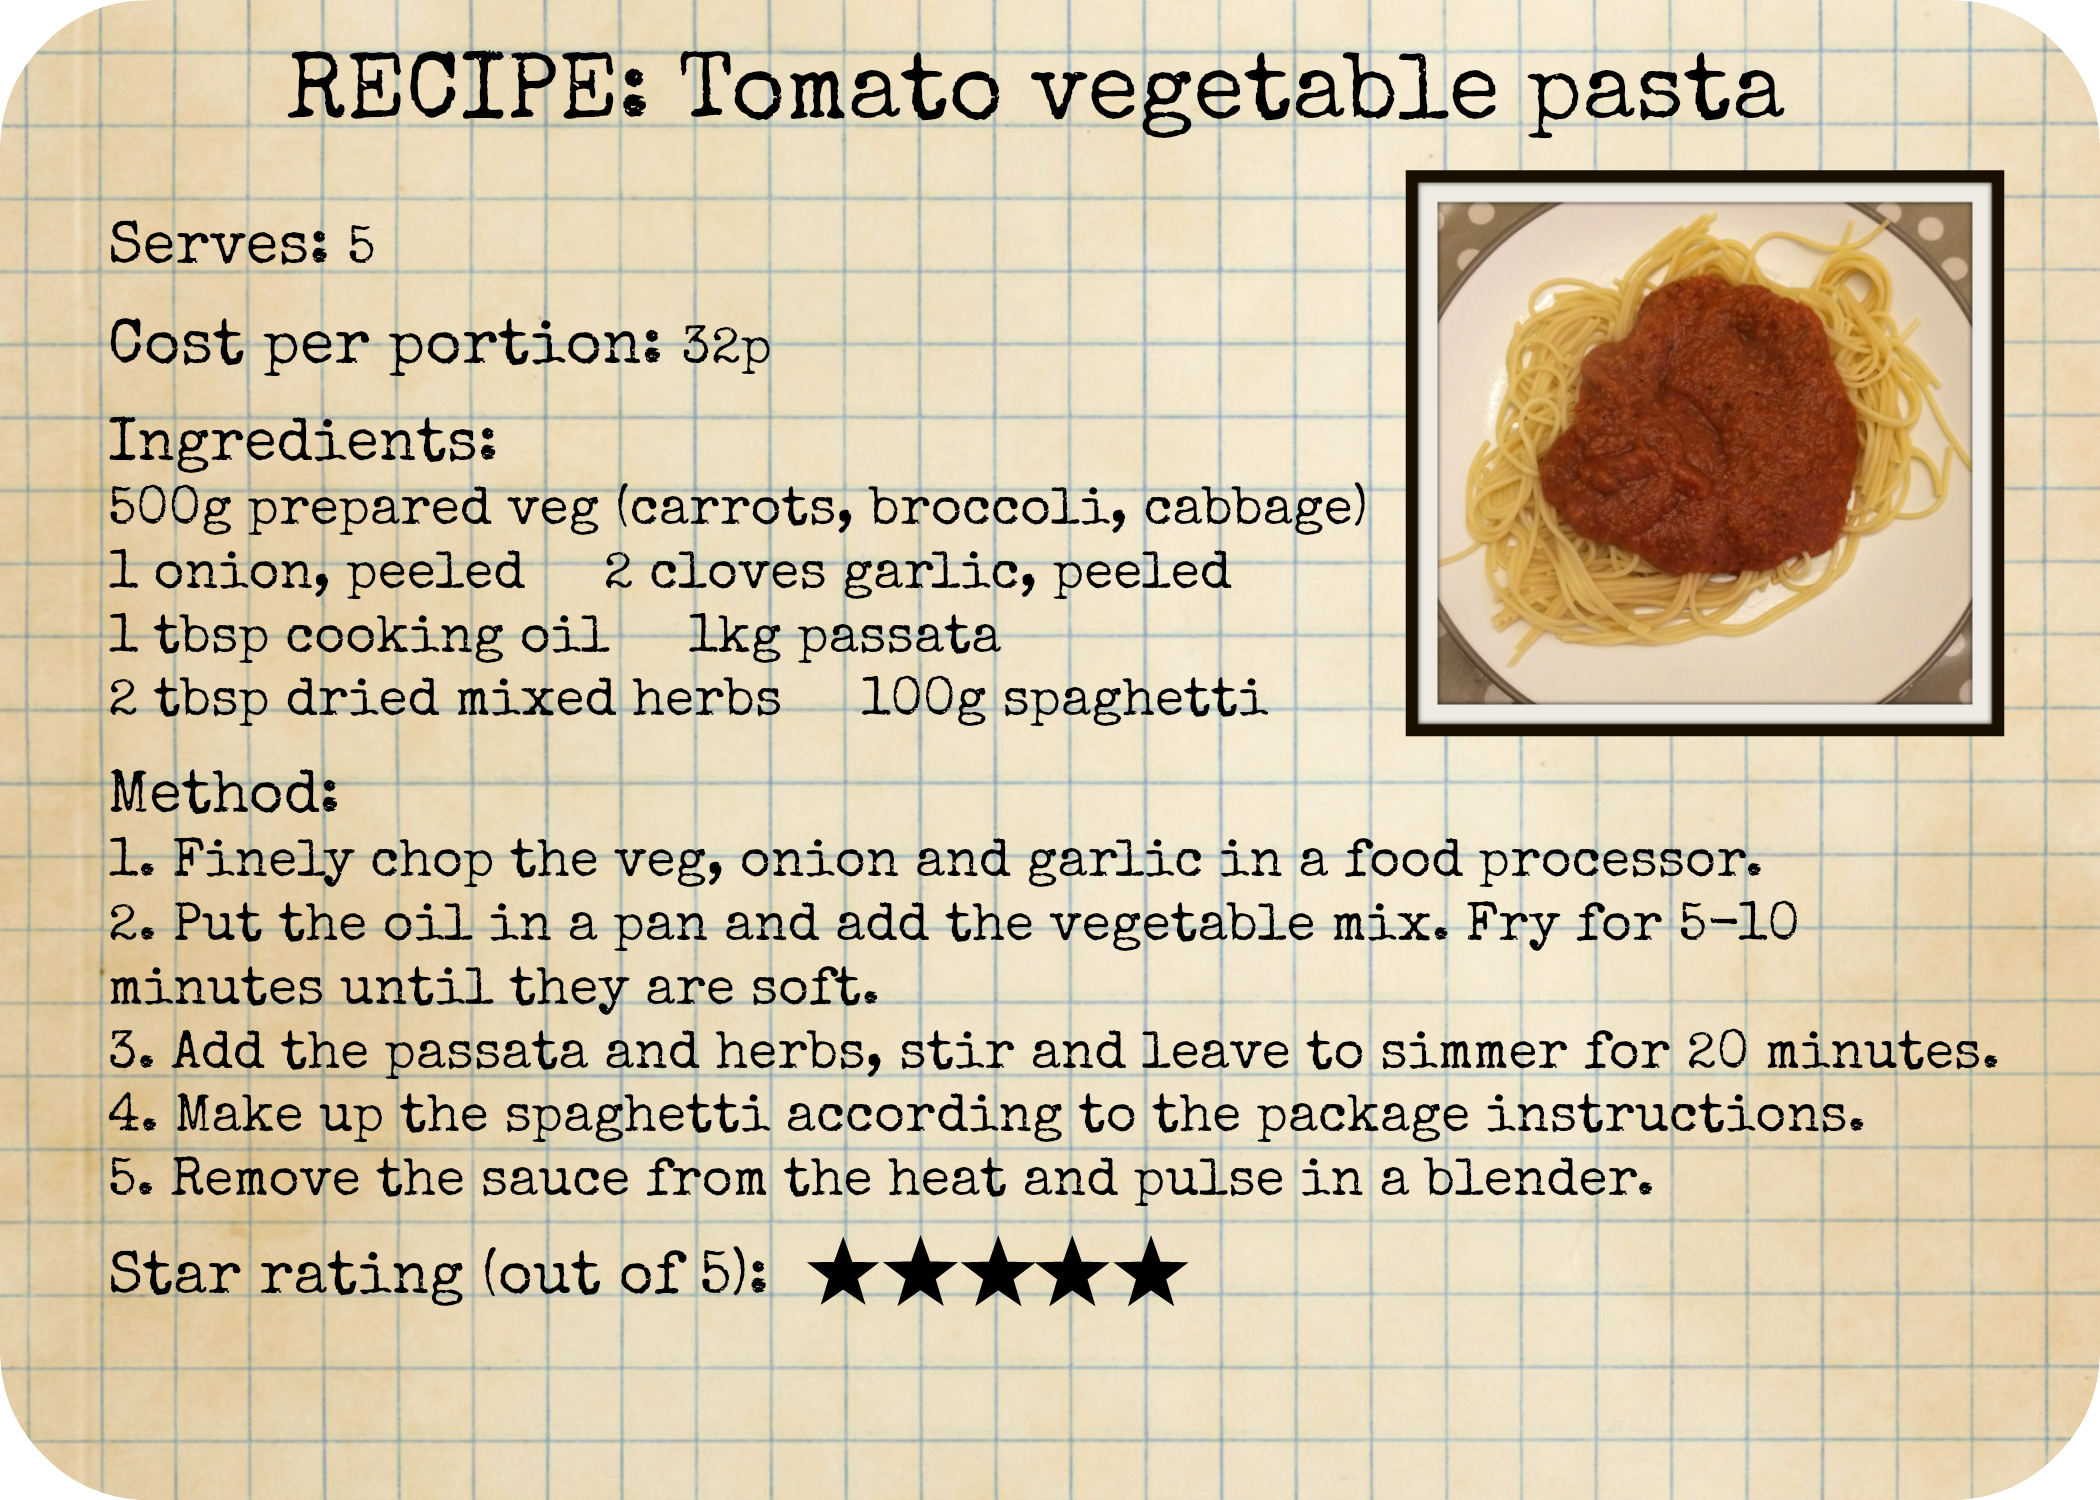
\includegraphics[scale=0.075]{recipe.jpg}
				\caption*{}
			\end{figure}
		}
		\only<4>{
			\centering What does this do?
			\begin{figure}[h]
				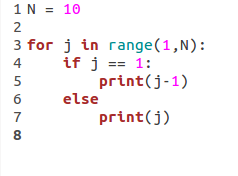
\includegraphics[scale=0.5]{python.png}
				\caption*{}
			\end{figure}
		}
	\end{column}
\end{columns}

\end{frame}

\begin{frame}{Computers Need Rules}

\begin{columns}	
	\begin{column}{0.5\textwidth}
		\begin{itemize}[<+->]
			\item Computers take an input, follow some rules, and give an output.
			\item Based on minimal input, computers can be \textit{trained} to excel at certain tasks.
		\end{itemize}
	\end{column}
	\begin{column}{0.5\textwidth}
		\begin{figure}[h]		
			\centering
			\animategraphics[controls,scale=0.25]{12}{animations/deepmind}{1}{365}
		\end{figure}
	\end{column}
\end{columns}

\end{frame}

\begin{frame}{Algorithmic Thinking}

\begin{columns}	
	\begin{column}{0.5\textwidth}
		\begin{itemize}[<+->]
			\item Break large problem into small tasks.
			\item Assemble small tasks to solve large problem.
		\end{itemize}
	\end{column}
	\begin{column}{0.5\textwidth}
		\begin{figure}[h]		
			\centering
			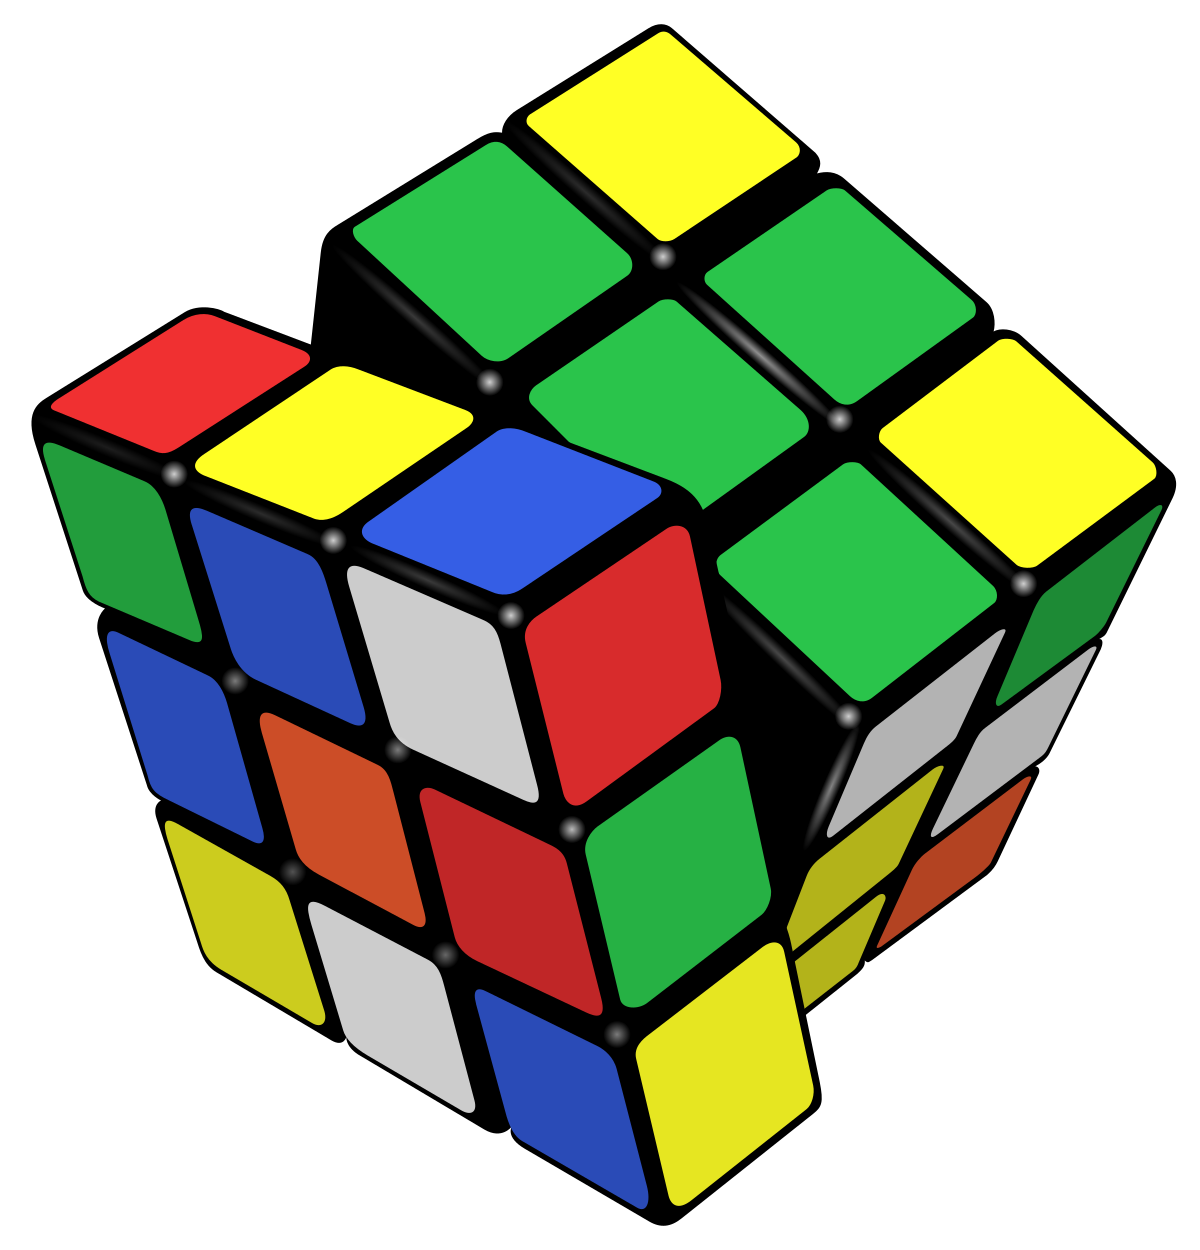
\includegraphics[scale=0.075]{rubiks.png}
			\caption*{}
		\end{figure}
		\only<3->{
		\begin{enumerate}[<+->]
			\item Solve top white face.
			\item Position corner pieces.
			\item Solve side faces.
			\item Solve underside.
		\end{enumerate}
		}
	\end{column}
\end{columns}

\end{frame}

\begin{frame}{Bugs are Everywhere!}
	
	\begin{columns}	
		\begin{column}{0.5\textwidth}
			\begin{itemize}[<+->]
				\item \textit{Debugging} is one of the most important parts of programming.
				\item To get good at debugging, you have to \textit{play}! Make mistakes, fix them, make more mistakes.
				\item \textbf{Making mistakes is how you learn here! No one (EVER) gets it right the first time!}				
			\end{itemize}
		\end{column}
		\begin{column}{0.5\textwidth}
			\begin{figure}[h]		
				\centering
				%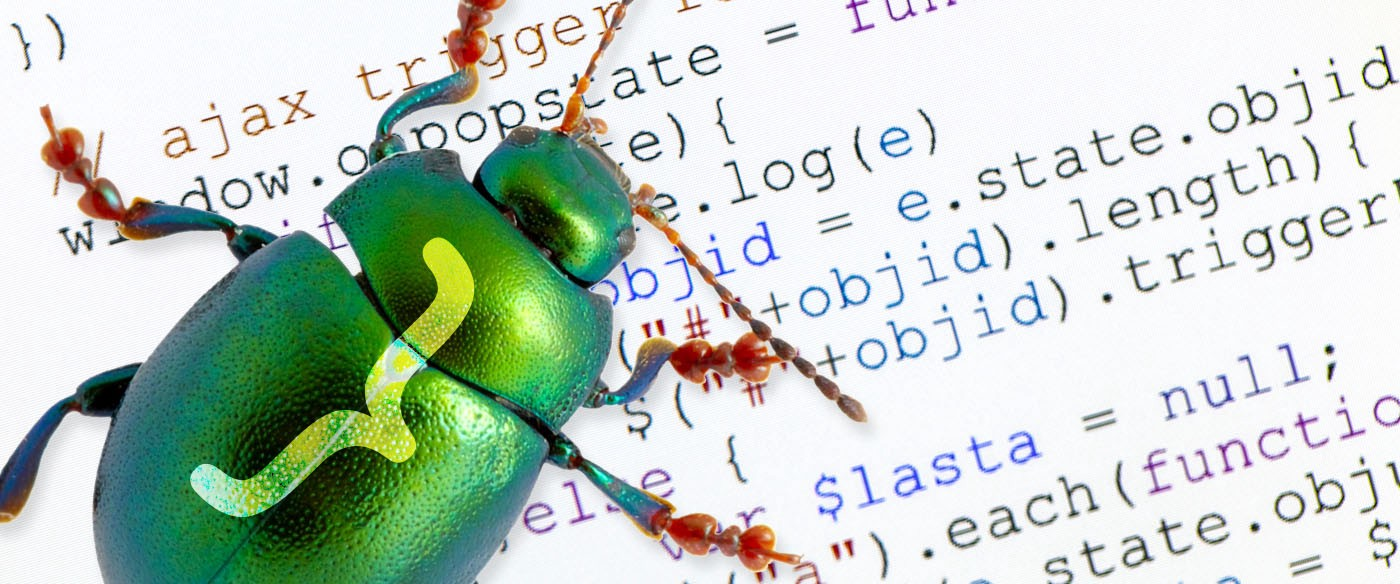
\includegraphics[scale=0.5]{debug.png}
				\caption*{}
			\end{figure}
		\end{column}
	\end{columns}
	
\end{frame}

\begin{frame}{Read - Search - Ask}	
	\only<1>{			
		\centering
		\huge \textbf{Read} - \textbf{Search} - \textbf{Ask} \normalsize
	}
	\only<2->{
		\begin{columns}
			\begin{column}{0.3333\textwidth}
				\centering \textbf{Read}
			\end{column}
			\begin{column}{0.3333\textwidth}
				\centering \textbf{Search}
			\end{column}
			\begin{column}{0.3333\textwidth}
				\centering \textbf{Ask}
			\end{column}
		\end{columns}
		\begin{columns}
			\begin{column}{0.3333\textwidth}				
				\begin{itemize}
					\item <2-> Read the documentation. 
					\item <3-> Does your program have a README file?
					\item <4-> Read the API (Application Programming Interface).
				\end{itemize}
			\end{column}
			\begin{column}{0.3333\textwidth}
				\begin{itemize}
					\item <5-> Google is your friend!
					\item <6-> More often than not, someone has already had your problem! 
					\item <7-> They've usually asked it on StackExchange.
				\end{itemize}
			\end{column}
			\begin{column}{0.3333\textwidth}
				\begin{itemize}
					\item <8-> \textbf{This is so important!}
					\item <9-> Collaboration and sharing ideas is how this field advances.
					\item <10-> Ask your friends, your teachers, the Internet.
					\item <11-> Use the \textit{gitter} chat for this!
				\end{itemize}
			\end{column}
		\end{columns}
	}
\end{frame}

\begin{frame}{Task}
	\begin{tcolorbox}[title=Experimenting with Python (15 mins)]
		Follow the instructions for Computaitonal Thinking - Lesson 1 at scott3142.com/btec
		\tcblower
		\textit{Experiment with the notebook. Change the variable names. Change the numbers. Play around. Make mistakes and fix them. Remember \textbf{Read-Search-Ask}!}
	\end{tcolorbox}
\end{frame}

\begin{frame}{Formulaic Thinking}
		
	\visible<1->{\centering \textbf{You will come across lots of formulae in this course!} \\}
	\visible<2->{\centering Don't freak out if you see them! \\}
	\visible<3->{\centering Approach them like a computer would! \\}
	\only<4->{
		\centering
		\begin{itemize}
			\item \textit{Break down into small pieces that are easy to manage.}
			\item \textit{Think logically!}
		\end{itemize}
	}
	
\end{frame}

\begin{frame}{Formulaic Thinking}

\begin{columns}	
	\begin{column}{0.5\textwidth}
		\begin{itemize}[<+->]
			\item What is the point of formulae?
			\item Where are they used in computing?			
		\end{itemize}
	\end{column}
	\begin{column}{0.5\textwidth}
		\visible<1->{
			\begin{align*}
				y &= mx + c \\
				x & = \frac{-b \pm \sqrt{b^2 -4ac}}{2a}
			\end{align*}
		}
		\visible<2->{
			\begin{align*}
				E &= mc^2 \\
				e^{i\pi} +1 &= 0
			\end{align*}
		}
	\end{column}
\end{columns}

\end{frame}

\begin{frame}{What's the Point of Formulae?}
	
	\begin{columns}	
		\begin{column}{0.5\textwidth}
			\begin{itemize}[<+->]
				\item $2^n - 1$				
			\end{itemize}
		\end{column}
		\begin{column}{0.5\textwidth}
			\begin{figure}[h]		
				\centering
				%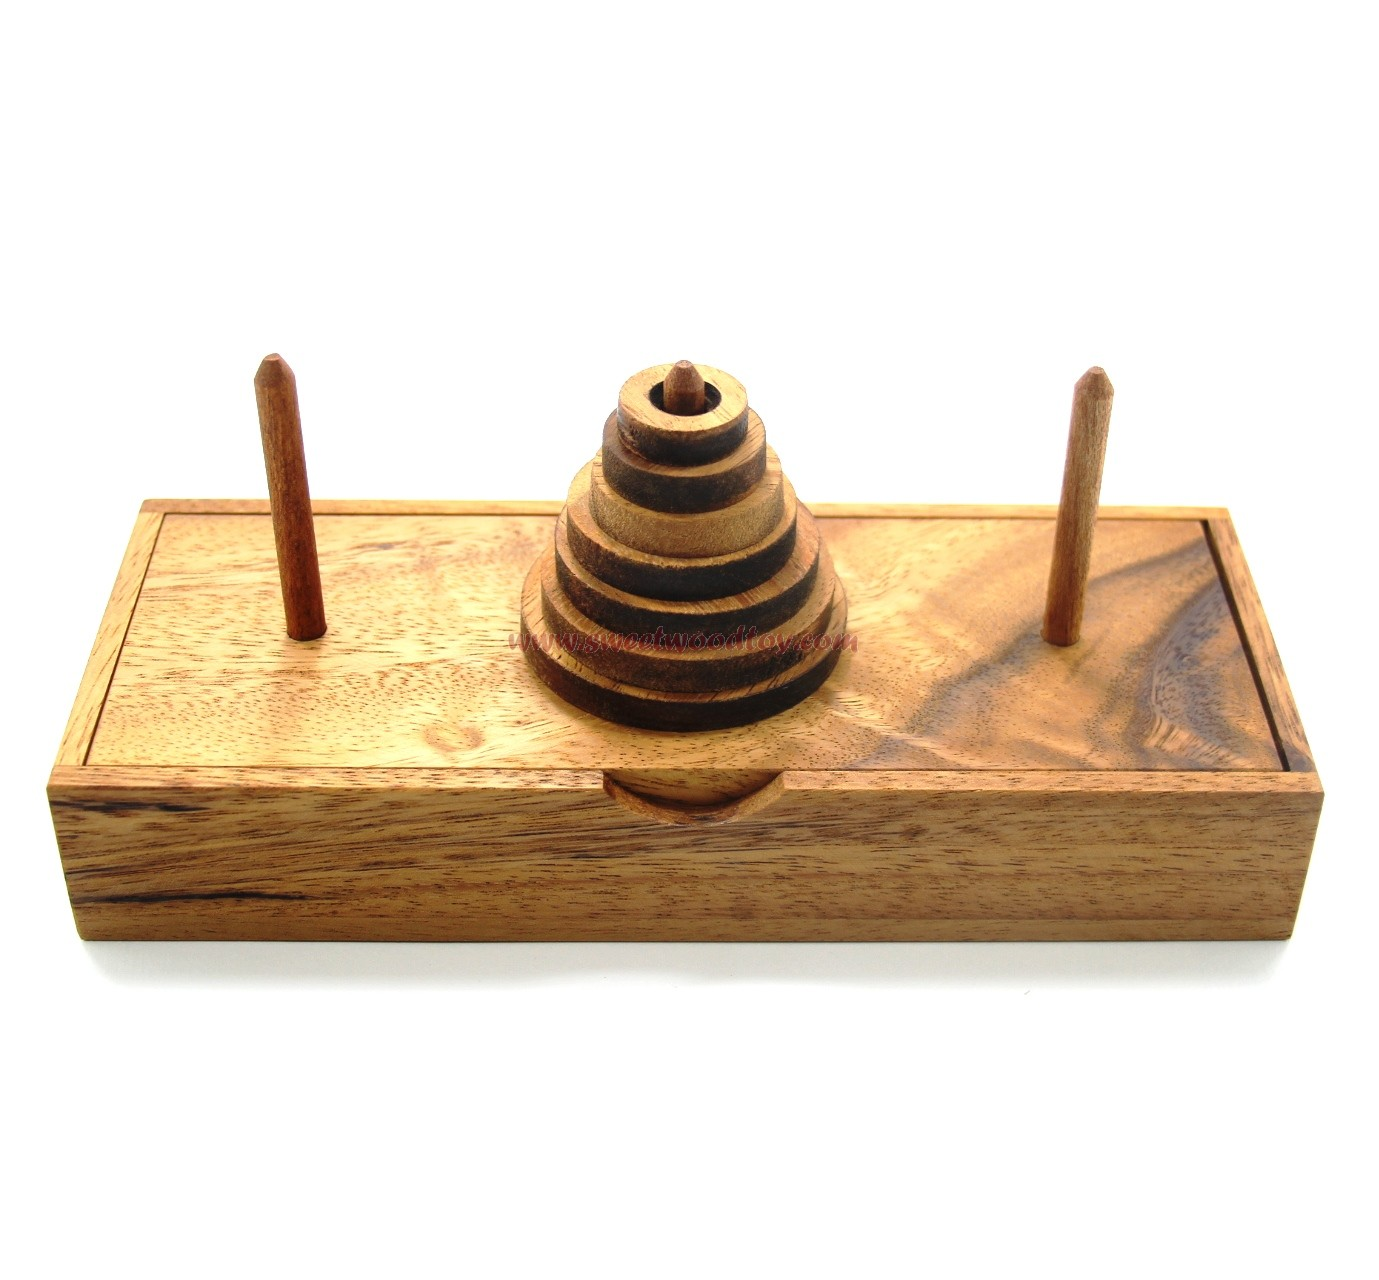
\includegraphics[scale=0.5]{hanoi.png}
				\caption*{}
			\end{figure}
		\end{column}
	\end{columns}

	\only<2->{
		\centering \textbf{Why is this important? What if we were writing code to solve this?}
	}
	
\end{frame}

\end{document}
